\begin{filecontents*}{\jobname.bib}
@article{Worsch_2009_AUC_ar,
  author  = {Thomas Worsch and Hidenosuke Nishio},
  title   = {Achieving universality of {CA} by changing the neighborhood},
  journal = {Journal of Cellular Automata},
  year    = {2009},
  volume  = {4},
  number  = {3},
  pages   = {237--246},
}
@inproceedings{Worsch_2012_IUA_ip_acri,
  author    = {Thomas Worsch},
  title     = {({I}ntrinsically?) Universal Asynchronous Cellular Automata},
  editor    = {Georgios Sirakoulis and Stefania Bandini},
  booktitle = {Proceedings ACRI 2012},
  year      = {2012},
  pages     = {689--698},
  publisher = {Springer},
  series    = {LNCS},
  volume    = {7495},
}
\end{filecontents*}

\documentclass[11pt,a4paper]{article}

\usepackage[T1]{fontenc}
\usepackage[ngerman]{babel}
\usepackage[utf8]{inputenc}

\usepackage{amsmath}
% \usepackage{mathtools}

\usepackage[tt=false]{libertine}   % !!!!! das muss man nicht nutzen
\usepackage[libertine]{newtxmath}  % !!!!! das muss man nicht nutzen
%\usepackage[supstfm=libertinesups,supscaled=1.2,raised=-.13em]{superiors} % params taken from doc

%
%\usepackage{tgpagella}
%\usepackage[euler-digits]{eulervm}
%
\usepackage{csquotes}

\usepackage{microtype}

\usepackage{fancyvrb}

\usepackage{graphicx}

\usepackage{booktabs}
\usepackage[shortlabels]{enumitem}
\setlist{noitemsep}

\usepackage{titlesec}
\usepackage{tcolorbox}
\tcbuselibrary{listingsutf8}

\usepackage{bbold}
\newcommand{\Z}{\mathbb{Z}}

\usepackage{hologo}

%-----------------------------------------------------------------------------
% für das Deckblatt

\usepackage{tikz}

\newcommand{\teilnehmername}{Klaus Philipp Theyssen} % !!!!!
\newcommand{\teilnehmermatrnr}{2061578}        % !!!!!
\newcommand{\seminarart}{Proseminar}           % !!!!!  oder Seminar
\newcommand{\seminarlp}{3 LP}                  % !!!!!  Prosem: immer 3 LP, Sem: 3 oder 4 LP
\newcommand{\seminarjahr}{2019}                % !!!!!
%-----------------------------------------------------------------------------
\newcommand{\meta}[1]{$\langle$\textit{#1}$\rangle$}
\newcommand{\paket}[1]{\texttt{#1}}
\newcommand{\prgname}[1]{\texttt{#1}}

%-----------------------------------------------------------------------------
\author{Klaus Philipp Theyssen}
\title{Proseminar Ausarbeitung Brown'sche Schaltkreise}

%=============================================================================
\begin{document}
%=======================================================================
% Anfang erste Seite
{\thispagestyle{empty}\large\sffamily\raggedright
%
\begin{tikzpicture}[remember picture,overlay]
  \coordinate[xshift=5mm,yshift=-5mm] (NW) at (current page.north west) {};
  \coordinate[xshift=-5mm,yshift=-5mm] (NE) at (current page.north east) {};
  \coordinate[xshift=-5mm,yshift=13mm] (SE) at (current page.south east) {};
  \coordinate[xshift=5mm,yshift=13mm] (SW) at (current page.south west) {};

  \draw[line width=0.25pt] (NW)
    [rounded corners=5mm] -- (NE) 
    [sharp corners] -- (SE)
    [rounded corners=5mm] -- (SW)
    [sharp corners] -- cycle
  ;
\end{tikzpicture}
%
\unskip % keine Ahnung warum das nötig ist
\noindent \textbf{\Large \seminarart\ (\seminarlp)} 
\\[\baselineskip]
%
Zellularautomaten und diskrete komplexe Systeme
% für Fortgeschrittene  % nur für das 4 Leistungspunkte Seminar !!!!!
\\[1ex]
%
im Sommersemester \seminarjahr

\vspace*{3\baselineskip}

\noindent \textbf{\Large Ausarbeitung} \\[\baselineskip]
%
von \textbf{\teilnehmername}, Matr.nr.~\teilnehmermatrnr

\vspace*{3\baselineskip}

\noindent \textbf{\Large Thema} \\[\baselineskip]
%
% nachfolgende ein Beispiel, für Konferenzbeiträge, Buchausschnitte, ...
% bitte analog vorgehen !!!!!
%
 Ferdinand Peper and Jia Lee (2018)\\[1ex]
%
\textit{On Non-polar Token-Pass Brownian Circuits}\\[1ex]
%
Reversibility and Universality, S.299-311
}
\clearpage
% Ende erste Seite
%=======================================================================
% Anfang zweite Seite
{\thispagestyle{empty}\raggedright

\noindent \textbf{\Large Erklärung}\\[1ex]
gemäß \S 6 (11) der Prüfungsordnung Informatik % !!!!! oder \S 6 (7) (bei MasterPO 2015)
(Bachelor) 2015 % oder Master !!!!!
\\[\baselineskip]

\noindent
Ich versichere wahrheitsgemäß, die Seminarausarbeitung zum
\seminarart{} "`Zellularautomaten und diskrete komplexe Systeme"' im
Sommersemester \seminarjahr{} selbstständig angefertigt, alle
benutzten Hilfsmittel vollständig und genau angegeben und alles
kenntlich gemacht zu haben, was aus Arbeiten anderer unverändert oder
mit Abänderungen entnommen wurde.

\vspace*{30mm}
\noindent
\begin{tabular}{@{}l}
  \hline
   \\[-1ex]
  \hbox to 0.6\textwidth{(\teilnehmername, Matr.nr.~\teilnehmermatrnr) \hss}
\end{tabular}
}
\clearpage
% Ende zweite Seite
%=======================================================================

%-----------------------------------------------------------------------------
\section{Einführung}
Aufgrund von geringerem Energieverbrauch in integrierten Schaltkreisen
werden in Zukunft Geräte von interesse sein die nur von einzelnen 
Partikeln geschaltet werden.
%
Dabei befinden wir uns nahe dem Thermalen Limit wobei die eigentlich
Energie zur Signalweiterleitung sehr klein ist und somit auch
Fluktuation ein Problem ist.
%
Die in diesem Paper präsentiereten Brown'schen Schaltkreise wollen
diese Fluktuation aktiv nutzen und sie zur Berechnung verwenden.


%-------------------------------------------------------------------------------
\section{Grundlagen}
Tokens sind diskrete nicht teilbare Einheiten die Signale modellieren.
%
Zunächst sind die einzelnen Schaltkreis Typen von einander zu unterscheiden 
und welche Unterschiede in Funktionalität existieren.
%
Allgemein sind alle hier vorgestellten Schaltkreise asynchron, dies bedeutet sie
haben keinen Zeitgeber und es kann nebenläufig zu Änderungen am Signal kommen.
%
Sie sind delay-insentive, was heißt das verzögerungen in der Signalweiterleitung
nicht zu unkorrekten Berechnungen führt.


\subsection{Token-based Schaltkreise}
Beispiel Petri netze (original Petri netze sind nicht turing complete aber 
es gibt erweiterungen die sie Turing complete machen) daher eher 
der Begriff Universell so verstehen, dass alle möglichen Schaltkreise
dieser Schaltkreisklasse mithilfe des T-Elements gebaut werden können.
%
Sie können von einer endlichen Menge an Schaltkreis Primitiven 
erzeugt werden (Merge, Fork, Tria)


\subsection{Token-pass Schaltkreise}
Äquivalenz von Token-pass und token-based zeigen (ein kabel wird zu zwei)
die entsprechenden TP-Merge, TP-Fork, TP-Tria.
%
Token-pass: \\
- keine Kabel \\
- miteinander Verbinden (kreuzend),\\
- keine Tokens Erzeugen

\subsection{Brown'sche Schaltkreise}
Die bisherigen Token-pass Schaltkreise können keine Deadlocks verhindern. 
%
Deshalb brauchen wir Fluktuation um die Deadlocks wieder aufzulösen mithilfe 
von Backtracking.

\subsubsection{Polare token-pass Schaltkreise}
In polaren token-pass Schaltkreises existiert eine bevorzugte Richtung
der Token, gekennzeichnet durch einen Pfeil.
%
Besonders bei den pre-Kabeln und post-Kabeln (also für Ein- und Ausgabe)
ist dies sinnvoll.

\subsubsection{Nicht polare token-pass Schaltkreise}
Hier können die Tokens frei fluktuieren, allerdings haben die T-Elemente eine
Einschränkung (kreise und blank symbole) wie sie Tokens verarbeiten.
%
Außerdem gibt es hier die möglichkeit von Terminatoren, dies sind Kabel
mit einem Ende auf dem Tokens sich einfach nur vor und zurück bewegen.
%
Die nicht-polaren Schaltkreise ermöglichen einfacheres Design und Verwendung
von weniger T-Elementen, weil bestimmtes Verhalten zum Verhindern von
Deadlocks nicht expizit modelliert werden muss.

%TODO T-Elemente bei Grundlagen mit einbauen und bei den jeweiligen 
%     Schaltkreis arten darauf verweisen
%-----------------------------------------------------------------------------
\section{T-Element}
Als Grundbausteine 

\subsection{Universalität}

%-----------------------------------------------------------------------------
\section{1-Bit Speicher}
Nun soll anhand eines 1-Bit Speichers die Funktionsweise von brown'schen 
token-pass Schaltkreisen erläutert werden. 

\subsection{Polarer token-pass 1-Bit Speicher}
Es werden 8 T-Elemente benötigt, es gibt ein Write und ein Read Bereich
es kann zu
%TODO was ist gemeint 
Überlaufen??!!
kommen beim schreiben.  

\subsection{Nicht polarer token-pass 1-Bit Speicher}
Es werden nur 7 T-Elemente benötigt auch, hier Konzept von Lesen und Schreiben
erklären und Bedeutung/ Nutzen von Terminator Kabeln.
Das Deadlock Backtracking zeigen.

%-----------------------------------------------------------------------------
\section{UND-Bauteil}
Als Teil meiner Eigenarbeit im Rahmen dieses Proseminars habe ich ein UND-Gatter
mithilfe von nicht-polaren T-Elementen entworfen.
%
Es benutzt den Deadlock backtracking Mechanismus und verundet ansonsten jede 
mögliche Eingabe mit jeder möglichen Ausgaben. 
%
Dabei werden zunächst T-Element zum modellieren der möglichen Wege benutzt, also 
das Token kann einen davon wählen, was wiederum der richtige ist oder zu einem Deadlock
führt. Solange bis sich beide Input Tokens "gefunden" haben.
%
Dann werden bei der C0 Ausgabe zwei Tokens benutzt um einfach die möglichen Wege zu 
verbinden.


\begin{center}
    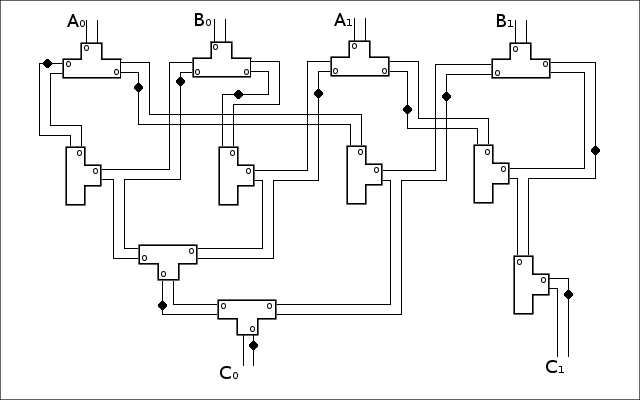
\includegraphics[width=15cm]{bilder/UndGatter.png}
\end{center}    

\subsection{Initialisierung}
Es ist eine Initialisierung auf der Abbildung gegeben (die Position der Tokens), 
außerdem ist sind die Kreise in den T-Elementen für eine korrekte Berechnung
elementar.
%
Diese Initialisierung ist natürlich nicht eindeutig und auch die Anordnung der Elemente 
ist veränderbar was die Funktion nicht beeinflusst.

\subsection{Korrektheit}
Eine interessante Frage ist nun ob die Korrektheit dieses Schaltkreises beweisbar ist. 
Wenn wir die angegebene Initialisierung vorraussetzen können, können wir uns die 
Korrektheit schnell klar machen indem :
%TODO mögliche Token interaktionen druchspielen OBdA für einen Fall



% ----------------------------------------------------------------------------
\section{Zusammenfassung und Ausblick}
In dem Paper (Non-polar token-pass Brownian Circuits) [1] wird eine neue Art
von Schaltkreis vorgestellt der zukünfitig in der Nanoelektronik eingesetzt
werden könnte.
%
Dabei ist das Konzept von Brown'scher Bewegung der Signale (Tokens) 
der interessante und neue Aspekt der es ermöglicht neue Arten von Schaltkreisen 
zu designen und auf ihre Eigenschaften zu untersuchen.
%
Jedoch sind Dinge wie Geschwindigkeit der Berechnung, Korrektheit beweisen und 
welche arten von konkreten Implementierungen möglich sind noch zu klären.


\section{Wann ist Berechnung vorbei?}

\subsection{Geschwindigkeit der Berechnung}

\subsubsection{Ein langes Kabel vs. viele T-Elemente}

\subsection{Implementierung}




\label{sec:summary}

Zum Abschluss kommt das Literaturverzeichnis.
%
Die beiden Zeilen

\begin{tcblisting}{listing only}
  \bibliographystyle{plain}
  \bibliography{\jobname}
\end{tcblisting}

erzeugen das, was man unter dieser Zeile sieht:

\bibliographystyle{plain}
\bibliography{\jobname}

\end{document}
